\section{土地金融}
\label{sec:92tudi}
\url{https://www.thepaper.cn/newsDetail_forward_11744994}


% 非常重要!!!!!!!!!!!!!
% !!\textbf{https://www.aisixiang.com/data/138457.html}
% \textbf{王小鲁:土地财政的昨天、今天和明天}

% https://pdf.dfcfw.com/pdf/H301_AP202305101586440193_1.pdf
% https://www.gov.cn/gzdt/2008-12/19/content_1182391.htm
% 刺破的泡沫—海南房地产往事  沈奇 杨政 https://www.sohu.com/a/761245832_482521
% 从沸腾到癫狂:泡沫背后的中国房地产真相
% 26年了,五届全国金融工作会议重大金融改革回顾(上)
% https://new.qq.com/rain/a/20231029A080O900

\subsection{海南房地产泡沫危机}
\label{subsec:hainan}


1988年8月23日,海南脱离广东省独立建省,并在海南设立经济特区。海南成为当时中国
最新、最大且是唯一的省级经济特区,成为全国各地淘金客们的狂欢
地。1989年到1993年间,商品房平均价格从1400元/平方米到7500元/平方米;商品房年
销售面积从1000万平方米到9000多万平方米;房地产投资总额从3.2亿元到93亿元;土地
价格从几十万元/亩到600万元/亩,


\begin{quotation}
  据太平洋证券数据,高峰时期,当时总人数不过656万的海岛上有两万多家房地产公司,
  平均每300个人一家房地产公司。与此同时,大量金融机构进入,海南短时间内成立
  了20家信托投资公司,35个城市信用社,此外还有一批股份制、会员制的金融性公司;
  证券行业从1989年初建立海南省证券公司,到后来已发展为26个证券机构34个证券交
  易点。\footnote{沈奇 杨政《刺破的泡沫—海南房地产往事》}
\end{quotation}
海南房地产此时玩的已经是金融“击鼓传花”游戏,下海官员、批条、虚拟概念(方案
和图纸)、信贷、炒楼花、炒地皮、炒项目,上一人传给下一人,死的是最后一个接盘
侠……

\begin{quotation}
  1993 年 6 月 23 日,时任国务院副总理的朱镕基发表讲话,宣布终止房地产公司上
  市、全面控制银行资金进入房地产业。24 日,国务院发布《关于当前经济情况和加强
  宏观调控意见》,\textbf{16 条}强力调控措施包括严格控制信贷总规模、提高存贷利率和
  国债利率、限期收回违章拆借资金、削减基建投资、清理所有在建项目等。银根全面
  紧缩,一路高歌猛进的海南房地产热顿时被釜底抽薪。这场调控的遗产,是给占全
  国 0.6%总人口的海南省留下了占全国 10%的积压商品房。全省“烂尾
  楼”高达 600 多栋、1600 多万平方米,闲置土地 18834 公顷,积压资金 800 亿元,
  仅四大国有商业银行的坏账就高达 300 亿元。
\end{quotation}

当时在海南炒房的“万通六君子”之一的潘石屹自述当时在泡沫破裂前成功抽身的原因:
\begin{quotation}
  我到海口规划局查了一下我们的项目,是有(证件)的。我这人特别好学习,除了看
  完自己的,我还要看看别的项目。

  我记得数字(海口规划局统计的海口人均住房面积)是四十九平方米。当时北京的人
  均住房面积是七点四平方米,而海南刚刚建省,在海口这样一个不富裕的地方,电都
  没有,一个红绿灯都没有的地方,建房子要接近五十平方米,北京才七平方米多。

  这就是房地产泡沫啊,跑的越早越好。于是我就赶紧跑到北京来,做了第一个项目,
  在阜成门这边,万通新世界广场,赚了不少钱。海口的企业家,多少企业家,基本上
  全军覆没,出来的很少。

  有好多人说,我们几个人,能够从海口这边逃着出来,能够从海南岛的92、93年房地
  产泡沫里逃着出来,非常聪明,很有远见。其实呢就是算数,就是建筑面积除一个人
  口数。就是常识。

  不要把这些商业的东西搞的多神秘,一会儿佛了,一会儿道了,一会儿鬼了,一会儿
  神了,没有这么神秘的东西,就是要尊重常识。
\end{quotation}
多么聪明,举一反三的潘石屹啊!你信么?反正笔者不信。


同期不止海南,北海、惠州、上海等地也出现了房地产热。朱镕基在1999年1月8日
在省部级领导干部金融研究班上对这时期的房地产热总结到:
\begin{quotation}
  从计划经济体制向社会主义市场经济体制过渡中,许多长期积累的深层次矛盾集中反
  映在金融领域。仅从房地产看,1992年、1993年的房地产热,就造成银行不良贷款几
  千亿元。目前,全国闲置的商品房多达7000多万平方米,价值在4000亿元左右;光是
  海南省就闲置1600万平方米,占压银行资金460亿元。原来占用的那些贷款,连本带息,
  现在要翻一番。同时,建起来的房子质量差、价格高,地理位置也不好,很难处理掉。
  这些绝大部分已成为银行的呆账、坏账。
\end{quotation}

沈奇、杨政:
\begin{quotation}
  海南烂尾房消化到2007年才接近结束。据泽平宏观数据,截至2006年10月,全省累计
  处置闲置建设用地23353.87公顷,占闲置总量的98.17%,处置积压商品房444.82万平
  方米,占积压总量的97.6%。而海南省的房价到2010年才再一次回到1993年时的水平,
  海南经济的萧条周期近20年。
\end{quotation}


\subsection{住房双轨制}
\label{sec:tudijnrong}


1990年5月19日国务院发布《城镇国有土地使用权出让和转让暂行条例》和《外商投资开
发经营成片土地暂行管理办法》,明确规定土地使用权可以采用\textbf{协议、招标和拍卖}三
种方式。“这标志着中国的土地市场走上了有法可依的轨道,从而使土地使用制度改革
在全国推开。”


1992 年 11 月,国务院发布《关于发展房地产业若干问题的通知》,提出进一步深化土
地所有制改革,继续深化城镇 居民住房制度改革。房地产的发展在 1992、1993 年迎来
了第一个高潮。1992、 1993 年商品房销售总额同比分别增
长 79.35\% 和 102.47\% ;1993 年固定投资完成额 累计同比始终保持在 60\%左右。

1993 年 6 月,国务院发布《国务院关于当前经济情况和加强宏观调控的意见》,提出
了“国 16 条”,即整顿金融秩序、加强宏观调控的 16 条政策措施。这是第一次国家
宏观调控过热房地产。其中包含要严控涉房信贷,坚决制止炒房地产获取暴利的行为,
房地产开发投资必须纳入固定资产投资计划等。海南房地产击鼓传花游戏走到尽头,泡
沫破灭。

经历初步探索之后,住房制度改革的市场化特征显现,逐渐形成以权力下放、培育市场
主体为特征的改革。1994年,国务院发布《关于深化城镇住房制度改革的决定》,提出
按照国家、企业和个人合理负担的原则进行住房体制改革,将公房实物分配改为\textbf{货币
  工资分配},建立\textbf{面对中低收入的保障性住房和面对高收入家庭的商品房},建
立\textbf{住房公积金}制度。至此,开始全面市场化的改革。\cite{CJZK201802012}

1994年这份《决定》并没有有效刺激房地产市场,当时东北国企已开始出现实质性大下
岗,全国主流仍是福利分房,毕竟机关事业和国企工作人员如果可以福利分房的话有多
少人会去市场买房呢?房地产市场尚不具备较大投资和金融价值。

据谢家谨《房地产这10年》回忆,
\begin{quotation}
  1996年7月11日,朱镕基在听取国务院房改领导小组汇报时指出:目前的宏观经济形势
  很好,是1993年以来最好的时期。但问题是国有企业亏损增加,经济效益下降;原因是结
  构不合理,企业生产的产品不适销对路;解决的途径是加大国有企业改革力度,调整产品
  结构,减少库存积压。关键是打开市场,搞活流通,培植\textbf{新的消费热点和经济增长点}。
  当前最有可能形成消费热点的是\textbf{房地产}……一要推进\textbf{住房商品化},二要有个好
  的规划。
\end{quotation}

1997年初中央决定继续实行适度从紧的财政货币政策。同年12月6日,国务院发布《关于
深化金融改革,整顿金融秩序,防范金融风险的通知》,提到“前些年出现的房地产热、
开发区热,造成大量不良信贷资产,其中大部分已成为呆账、坏账,无法收回”。


\subsection{新的增长点——住房市场化、资本化}


1997年东南亚金融危机已开始影响我国,1998年累计下岗近3000万人导致消费低迷,初级产
品出口出现负增长,形势严峻,财政紧缩尚未实施多少时日,便转为宽松,\textbf{此后财政
  货币政策时常在一两年、甚至两三个月内经历从决定紧缩到重返放宽的过程。}


1998年3月19日九届全国人大一次会议举行的记者招待会上,朱镕基说到:
\begin{quotation}
  我们必须确保今年中国的经济发展速度达到8\%,通货膨胀率小于3\%,人民币不能贬
  值……我们实现这些目标的主要手段是提高国内的需求……拿出较多的财力来刺激国
  内需求。这个需求就是加强铁路、公路、农田水利、市政、环保等方面的基础设施建
  设,加强高新技术产业的建设,加强现有企业的技术改造,当然还有住房建设,因为
  这是中国国民经济的新增长点。


  第三是住房制度改革。住房的建设将要成为中国经济新的增长点,但是我们必须把现
  行的\textbf{福利分房政策改为货币化、商品化的住房政策},让人民群众自己买房子。整个房
  改方案已酝酿三年多。我们准备今年下半年出台新的政策,停止福利分房,住房分配
  一律改为商品化。
\end{quotation}

1998年5月,《个人住房贷款管理办法》发布。7 月,国务院发布《关于进一步深化城镇
住房制度改革加快住房建设的通知》,正式宣布\textbf{1998年下半年开始停止住房实物分配
  (停止福利分房),逐步实行住房分配货币化} ;建立和完善\textbf{以经济适用住房为主}的
多层次城镇住房供应体系;\textbf{发展住房金融},培育和规范住房交易市场。

据1998年3月任财政部部长的项怀城回忆,原定\textbf{5年内消化470亿元财政赤字}的财政紧缩预
想被打乱。同年8月份,财政部执行1997年3月1日人大委员会通过的决议,发行期限
为\textbf{30年的2700亿元特别国债(不计入赤字)},向四大国有商业银行定向发行,所筹资
金专项用于补充四大银行资本金,以达到国际清算银行《巴塞尔协议》要求——银行资
本充足率不得低于8\%,挽救了濒临技术性破产的国有四大行。此外财政部又增
发\textbf{1000亿元10年期长期建设国债}(其中500亿元计入中央财政支出;另外500亿元算作
中央替地方发债,转拨地方,\textbf{地方这500亿元不计入赤字}。),银行据此再
发\textbf{1000亿元贷款}。根据项怀城主编的《中国财政通史》,“1998--2004年共发行\textbf{长
  期建设国债9100亿元}”。


原本1997年4月发布的《中共中央、国务院关于进一步加强土地管理切实保护耕地的通知》
中规定“农地转为非建设用地的土地收益,全部上缴中央”。经过一年多中央和地方博
弈,被1998年8月29日修订通过,1999年1月1日起实施的《土地管理法》“新增建设用地
的土地有偿使用费,30\%上缴中央财政,70\%留给地方人民政府”所取代。中央希望通
过土地收益方案的调整,来加强土地管理和耕地保护工作,但在地方政府的强烈反对下
未能实现。\cite{ZDJJ200804009}

另外,《土地管理法》第二条规定“国家为公共利益的需要,可以依法对集体所有的土地实行
征用”,农业用地如想变为建设用地,需经过征地环节,只有变成国有土地后才能上市
转让,这也就确立了政府对于建设用地的垄断地位。

% 朱镕基
% \begin{quotation}
%   我国金融领域风险究竟是怎么造成的?其中原因很多,主要有以下四个方面。

%   首先是历史遗留的问题。从计划经济体制向社会主义市场经济体制过渡中,许多长期
%   积累的深层次矛盾集中反映在金融领域。仅从房地产看,1992年、1993年的房地产热,
%   就造成银行不良贷款几千亿元。目前,全国闲置的商品房多达7000多万平方米,价值
%   在4000亿元左右;光是海南省就闲置1600万平方米,占压银行资金460亿元。原来占用
%   的那些贷款,连本带息,现在要翻一番。同时,建起来的房子质量差、价格高,地理
%   位置也不好,很难处理掉。这些绝大部分已成为银行的呆账、坏账。目前政策性银行
%   的风险也很大。粮棉收购贷款长期被严重挤占挪用,大量的亏损在银行挂账。国家开
%   发银行一个报告反映,煤炭建设项目所形成的不良贷款,不但使煤炭行业陷入困境,
%   也对开发银行的生存和发展构成严重威胁。

%   二是重复建设。多年来盲目上项目,搞了大量的重复建设,又主要是靠银行贷款,许
%   多企业借银行钱的时候就根本没有想到要还。前些年银行固定资产投资贷款利率
%   在10\%以上,什么项目有这么高的回报率?不少项目建成之日就是亏损之时。例
%   如,90年代初期,全国一下子上了十几套小乙烯项目(年产11.5万吨)。小乙烯成本高,
%   产品单一,没有销路。广州小乙烯投资花了80多亿元,投产后一年就得亏损几亿元。
%   重复建设不仅形成了巨额银行不良贷款,也造成大量的重复生产,而靠银行流动资金
%   贷款生产出来的产品没有市场,积压在仓库里,企业亏损又都挂在银行账上。

%   三是行政干预。一些地方和部门的领导干部,缺乏金融知识,不懂金融法律、法规,
%   随意干预银行和其他金融机构的正常经营活动,把金融机构贷款当做财政的钱来花。
%   前些年,许多地方搞“现场办公会”、“资金调度会”,往往都是指令银行或其他金
%   融机构贷款。缺乏市场调查,缺乏科学决策,结果不少贷款都投向了没有市场、没有
%   效益、没有还贷能力的项目,大都是有去无回;甚至还有相当部分资金被用于盖办公
%   大楼、发奖金和政府行政开支,最后都形成了金融不良资产。广东省恩平市原领导班
%   子肆意干预金融活动,造成80多亿元的金融资产损失,就是一个很典型的事例。最近
%   一个时期,一些地方刮起出售国有小企业之风,搞所谓“一卖了之”。名义上卖,实
%   际上是半卖半送,甚至是明卖暗送,许多银行的贷款都被冲掉了。工商银行去年搞了
%   一次检查,发现在企业“改制”中悬空和逃废该行债务有1000多亿元。

%   四是金融系统腐败现象严重。许多银行和其他金融机构严重违法违规经营,高息揽储,
%   搞账外经营,谋取小团体甚至是个人私利,造成许多资金收不回来。一些金融从业人
%   员素质不高,以权谋私,内外勾结,营私舞弊,腐化堕落,使大量金融资产流失。对
%   金融系统中的腐败行为,我们虽然一直采取严厉的惩处措施,但这些年金融案件仍屡
%   屡发生。

%   当前我国金融领域的问题确实比较严重,防范和化解金融风险的任务也十分艰巨,但
%   信心绝不可动摇。我们完全有条件、有办法、有能力解决所面临的问题。20年来的改
%   革和发展奠定了良好的基础,经济实力比较雄厚,当前宏观环境比较宽松,重要产品
%   和外汇储备充足,党中央有驾驭复杂局势的能力,我们也积累了一些化解金融风险的
%   经验。正确认识问题所在,也是解决问题的必要条件。充分运用这些有利条件,我们
%   就能够抵御任何风险,战胜任何困难。因此,我们在看到问题和困难的时候,更要看
%   到光明,鼓起勇气,增强信心。当然,从根本上解决金融领域的问题,绝非轻而易举,
%   需要全党、全国上下齐心协力,同舟共济。
% \end{quotation}

\subsection{土地招拍挂}
据王永红:
\begin{quotation}
  有媒体透露,1987年至1999年,深圳市利用拍卖和招标两种方式一共卖出了80多宗地,
  面积基本上都在1万平方米左右。而每年协议出让面积是100多万平方米。两者相差甚
  远。1995年、1996年还一度终止了土地拍卖。1997年连一次招标或拍卖都没有举
  行。1998年深圳市土地出让金达108亿元,但这一年仅有的两次招标和两次拍卖,一共
  只有3.3亿元。1999年之前,深圳90\%的土地实行的是非市场价格的协议出让。

  协议出让意味着存在很强的人为操纵的可能性。让行政权力从富有诱惑力的利益空间
  中退出,发挥市场机制在土地资源配置的基础性作用,需要很大的勇气,但能带来巨
  额的回报。1999年,浙江开始在全省范围内实行\textbf{经营性用地一律招标拍卖制
    度}。2000年,全国土地招标拍卖收益为350亿元,而浙江一个省就达195亿元。

  基层的首创精神,在2001年国务院15号文件(即《关于加强土地资产管理的通知》)
  和2002年国土资源部11号令(即《招标拍卖挂牌出让国有土地使用权规定》)中受到
  了高度重视。国务院15号文件提出,从严格控制建设用地供应总量,严格实行国有土
  地有偿使用制度,大力推行\textbf{招标拍卖},加强土地使用权转让管理,加强地价管理和
  规范土地审批行为。国土资源部11号令则\textbf{对经营性土地协议出让“叫停”},明
  确\textbf{四类经营性用地使用权出让必须采用招拍挂方式}。这两个文件对土地市场建设的
  推进作用显而易见:2000年全国招标拍卖出让土地的收益为350亿元,2001年为492亿
  元,增长率为40\%。2002年,全国国有土地使用权招标拍卖挂牌出让的宗数、面积、
  价款分别是上年的108.55\%、273.8\%和197\%。
\end{quotation}

土地的市场化、资本化价值大幅上升,但当时房地产商自然仍倾向于低价的协议拿地,
或者也缺乏与招拍挂相应的庞大资金,地方政府为了房地产商可以多拿地及协议转让大
幅权力寻租空间与之媾和,不管是出让土地面积还是出让收入,仍以协议出让为主。

国土资源部15号文落款日期为2002年5月9日,要求7月1日起施行。北京市就抢于6月28日
发文《关于停止经营性项目国有土地使用权协议出让有关规定的通知》(京政办
发[2002〕33号),开了几个允许\textbf{协议转让}的口子,如“绿化隔离带项目、小城镇建
设项目、危旧房改造项目以及其它重大建设项目中的经营性项目用地”(被称为“四个
口子”,“属于规划为高科技、工业用途的经营性项目用地确需协议出让的。”

\begin{quotation}
2004年3月31日,国土资源部、监察部发出《关于继续开展经营性土地使用权招标拍卖挂
牌出让情况执法监察工作的通知》,要求对土地出让的所有历史遗留问题,必须
在2004年8月31日前界定并处理完毕。\textbf{8月31日后,不得再以历史遗留问题为由采用协议
方式出让经营性土地使用权。}业内称之为“\textbf{8·31大限}”。国土资源部为此多次召开座谈会
和电视电话会议作出部署。也就是2004年9月1日以后,土地使用权招标拍卖挂牌制度
(简称土地招拍挂制度)得以在全国建立。
\end{quotation}

既然中央强令,而招拍挂确实可让地方政府获得更多土地转让收入,那地方何乐而不为
呢?

地方政府原来主要是低价或零低价出让工业用地,以吸引外来投资、刺激经济发展、扩
大GDP考核指标;自招拍挂制度建立后向低价征地、高价出让住宅、商业用地发展,以赚
取高额利差。“\textbf{从此开发商(消费者)之间为买地而展开竞争,政府(生产者)坐享生产
者剩余。土地成为地方政府最主要的资本来源}”\cite{dajueqi}。

招拍挂和协议出让历年比例变化请见\cref{tab:zhaopaigua}。
% Please add the following required packages to your document preamble:
% \usepackage{booktabs}
% \usepackage{multirow}
% \usepackage{graphicx}
\begin{table}[]
\centering
\resizebox{\textwidth}{!}{%
\begin{tabular}{@{}llllllllll@{}}
\toprule
\multirow{2}{*}{年份} & \multicolumn{4}{l}{出让土地面积比重} &  & \multicolumn{4}{l}{出让收入比重} \\ \cmidrule(l){2-5}  \cmidrule(l){6-9}
                    & 协议    & 招标    & 拍卖    & 挂牌   &  & 协议    & 招标   & 拍卖   & 挂牌   \\ \midrule
2002                & 0.84  & 0.03  & 0.10  & 0.02 &  & -  & - & - & - \\
2003                & 0.72  & 0.03  & 0.05  & 0.19 &  & 0.43  & 0.12 & 0.16 & 0.29 \\
2004                & 0.71  & 0.02  & 0.05  & 0.21 &  & 0.45  & 0.08 & 0.15 & 0.33 \\
2005                & 0.65  & 0.03  & 0.06  & 0.26 &  & 0.29  & 0.08 & 0.16 & 0.48 \\
2006                & 0.69  & 0.01  & 0.05  & 0.24 &  & 0.28  & 0.04 & 0.16 & 0.52 \\
2007                & 0.50  & 0.01  & 0.06  & 0.43 &  & 0.18  & 0.04 & 0.21 & 0.58 \\
2008                & 0.16  & 0.02  & 0.06  & 0.76 &  & 0.07  & 0.05 & 0.13 & 0.74 \\ \bottomrule
\end{tabular}%
}
\caption{不同土地出让方式出让土地面积、收入的构成}
\label{tab:zhaopaigua}
\capsource{来源:李郇、洪国志、黄亮雄《中国土地财政增长之谜》}
\end{table}

王永红《攀登新的高度——我国土地有偿使用制度改革30年历程》:
\begin{quotation}
一些地方为招商引资,工业用地出让中长期存在着低地价乃至“零地价”行为,严重干
扰了土地市场秩序,为一些地方搞低水平重复建设和扩大固定资产投资提供了条件。其
获取土地的方式必须加以改革。国务院15号文件已经提出:除按现行规定必须实行招拍
挂的土地外,工业用地也要创造条件逐步实行招拍挂出让。这个规定是工业用地进入招
拍挂的一个信号。

2004年出台的《国务院关于深化改革严格土地管理的决定》(即国务院28号文件),有
针对性地指出:“必须严禁非法压低地价招商”,同时要求要加快探索和实践,加快工
业用地进入市场化配置。2006年出台的《国务院关于加强土地调控有关问题的通知》
(即国务院31号文件),则完全把工业用地纳入了市场竞争的范围,要求“工业用地必
须采用招标拍卖挂牌方式出让,其出让价格不得低于公布的最低价标准” 。

2006年12月27日,国土资源部发布《全国工业用地出让最低价标准》,并将
从2007年1月1日起实施。此举标志着,我国工业用地必须采用招标拍卖挂牌方式出让,
其出让底价和成交价格均不得低于所在地土地等别相对应的最低价标准。

工业和经营性用地招拍挂出让,由国家政策上升为国家法律。2007年3月16日颁布的《物
权法》明确规定:“工业、商业、旅游、娱乐和商品住宅等经营性用地以及同一土地有
两个以上意向用地者的,应当采取招标、拍卖等公开竞价的方式出让。”
\end{quotation}

\subsection{土地增值税}

\begin{quotation}
  土地增值税(采用累进税率)在一定程度上能够体现土地级差地租和增值收益……国
  家征收土地增值税,主要目的是为\textbf{调节房地产开发市场的秩序,抑制房地产开发、
    转让的暴利行为}。因此,这一税种的征收,最主要受到影响的还是房地产开发企业,
  特别是开发别墅、公寓、写字楼等高档项目的开发商,以及炒卖楼花的个人买卖行
  为。\cite{yangdi}
\end{quotation}

土地增值税在1994年分税制后属于地方政府收入,但一直征收不利。国家税务总局
自2005年至2010年,曾经8次发文,对土地增值税的预征和清算提出要求,各地进展甚微。
包括房地产上市公司在内,地产商一般是以1\%的预征率来进行土地增值税的计提,远远
低于实际清算的税率。地产商出现拖欠、不清算、不缴纳土地增值税、甚至开发后注销
公司等现象。地方政府碍于地产商提供的大额土地转让金及其他财政贡献,往往对占小
头的土地增值税消极作为。而中国财政金融压力甚或危机有时也使严格清算土地增值税政
策半途夭折。

\begin{quotation}
《21世纪经济报道》记者荆宝洁曾获得一份未公开的政协提案。一位不愿透露姓名的全
国政协委员在这份提案中说,根据计算,2005年到2009年土地增值税共流失2.52万亿元。

对土地增值税的严格预征和清算,不足以让地方政府放弃对土地财政的依赖,原因仍然
是土地收入太过巨大,其他收入无可替代。不过,中央政府愿意为地方政府寻找新的收
入来源,地方政府当然会笑纳。\cite{2011feiteng}
\end{quotation}

\subsection{地产商阶层对金融监管的胜利}

中国人民银行办公厅2003年6月6日印发《关于进一步加强房地产信贷业务管理的通知(银发
〔2003〕121号):
\begin{quotation}
  通知规定:

  商业银行严禁以房地产开发流动资金贷款及其他形式贷款科目发放房地产开发贷款,
  并要求\textbf{企业自有资金不低于开发项目总投资的30\%;对土地储备机构发放抵押贷款,
    贷款额度不得超过所收购土地评估价值的70\%,贷款期限最长不得超过2年};对未
  取得土地使用权证书、建设用地规划许可证、建设工程规划许可证和施工许可证的项
  目,\textbf{不得发放任何形式的贷款};商业银行发放的房地产贷款,\textbf{严禁跨地区使用};商业
  银行不得发放用于缴交土地出让金的贷款。

  \textbf{商业银行只能对购买主体结构已封顶住房的个人发放个人住房贷款};对借款人申请个
  人住房贷款购买第一套自住住房的,首付比例仍执行20\%的规定;“对购买第二套以
  上(含第二套)住房的,应适当提高首付款比例”;“个人商业用房贷款的抵借比不
  得超过60\%,\textbf{贷款期限最长不得超过10年,并且所购商业用房为竣工验收的房屋}”。
  (人民银行提供)
\end{quotation}

时任金融监管机构——中国人民银行货币政策司司长的戴根有被认为是起草121号文件的
关键人物。据他自述2001年就注意到房地产市场一些局部问题,其2002年向人行领导汇
报“\textbf{一是房地产投资增长明显高于销售的增长,第二是商品房空置面积明显增长,而且
增长幅度非常高}。因而给出了“部分地区房地产出现过热”的判断意见。”2002年4季度
抽查商业银行房地产信贷情况发现,房地产信贷违规金额接近\sfrac{1}{4}。\footnote{21世纪新闻报
  道,\href{https://finance.sina.com.cn/x/20031101/1105501003.shtml}{121文件
    内幕 戴根有回应:谁说121与18矛盾?}}

121号文件受到很多大房地产商的声讨和行动抵
制\footnote{https://news.sina.com.cn/c/2003-09-16/14051753586.shtml}。两个多月后《国
务院关于促进房地产市场持续健康发展的通知》(国发〔2003〕18号)出台,提到“房
地产业关联度高,带动力强,已经成为\textbf{国民经济的支柱产业}”“\textbf{发展住房信
  贷}”“\textbf{建设部要会同有关部门……指导各地具体实施并负责对本通知贯彻落实情况
  的监督检查。}”。

地产商冯仑就此说到“\textbf{商人的声音首次大过了政府的声音}”,一些评论家认为这
是“\textbf{地产商阶层的胜利}”。10月份,戴根有调任中国人民银行征信管理局局长。



% 2003年6月25日,时任国家审计署审计长的李金华作2002年年度审计报告时提到:
% \begin{quotation}
%   (2001)年抽查建行广州地区8家支行的楼宇按揭贷款,发现有\textbf{10亿元是虚假按揭},
%   有的不法分子甚至内外勾结,骗取银行资金。如广东省汕尾市公安局某副局
%   长,1998至1999年,冒用他人名义,出具虚假证明,骗取建行广州市芳村支行按揭贷
%   款3793万元,有3270万元已无法追回,其中转入该副局长等人个人账户的2576万元全
%   部被提取现金,去向不明。目前,该副局长等9名犯罪嫌疑人已被公安机关拘捕。
% \end{quotation}



2005年8月15日,央行金融市场司房地产金融分析小组在发布的《2004中国房地产金融报
告》中提出,“很多市场风险和交易问题都源于商品房新房的预售制度,目前经营良好
的房地产商已经积累了一定的实力,可以考虑\textbf{取消现行的房屋预售制度},改期房销售
为\textbf{现房销售}”。

房地产商们多以现房销售将引起房价上涨为理由反对现房销售。笔者认为,真实原因显
而易见,资本只有自我增殖这一本质目的,现房销售将引起房地产大幅降杠杆,资金流
也随之匮乏干涸,金融属性大幅削弱才是真正原因,房价上涨是这一真正原因的副作用而已。

袁一泓\cite{2011feiteng}写到:
\begin{quotation}
  2005年8月24日,\textbf{建设部}新闻发言人表示,商品房预售制度是《城市房地产管理法》
  确立的一项制度。从十多年的实践看,这一制度与我国国情是适应的,目前还不能取
  消。

  \textbf{地产商们又赢了。}
\end{quotation}



据21世纪新闻报道\footnote{\url{https://news.cctv.com/financial/20080326/100431.shtml}},
\begin{quotation}
  国家审计署2007年第86号《上海市社保基金运营及管理情况专项审计》报告所披露的
  社保基金整体状况远比此前所暴露的福禧个案更为触目惊心:"多年来,上海市社保局共
  计运营基本社会保险基金、企业年金、小城镇保险等8个险种的社保资金,金额共计
  达329.44亿,截至2006年7月17日,尚未收回的资金达255.41亿,占运营资金余
  额387.31亿元的66\%。"

  根据报告,这些违规运营的社保资金大量投向了和国家宏观政策导向不符的产业领
  域——比如房地产业。

  "截至2006年7月17日,\textbf{对44家房地产企业贷款余额201.25亿,社保资金甚至给不法商
    人和企业提供了大量的资金支持。}"
\end{quotation}

养老金个人账户依照1997年《国务院关于建立统一的企业职工基本养老保险制度的决定》
要求,应是实收账户——账钱相符、账人相符、账账相符,但历年来被一些地方政府挪
用至养老金统筹账户或者搞金融投资、基建和房地产,具体数字不可考。其后二十年,国
务院数次要求坐实养老金个人账户,但最终未见实效。2010年代末可能不少地区已直接
转为名义账户——只记帐面数字,不做实,没有真实资金。
\begin{quotation}
  首先,名义账户制度下个人的养老金待遇完全由个人缴费水平决定,因此失去了在参
  保者之间进行收入再分配的功能,这从根本上动摇了国家基本养老保险制度的互助共
  济性与公平性。

  其次,名义账户制度下由于缴费率确定不变,养老金水平下降之势几乎不可逆转。

  再次,由于名义账户制下影响记账利率的因素是多元的,养老金增长率的波动性增大,
  结果必然削弱基本养老保险制度的稳定安全预期。\cite{mingyizhanghu}
\end{quotation}


2006 年在国内房价高启、地产行业景气上升的大背景下,房地产上市公司的盈利能力超
过了 A股市场的平均水平。共实现主营业务收入 927.48 亿元,净利润 83.36 亿元;同
比增长接近 30\%和 60\%。\footnote{据水清木华研究中心《2006-2007 中国房地产业上市公司
  研究报告》}

2007年全国共完成房地产开发投资额25280亿元,增长30\%,增速上升7.4个百分点,高
于其他行业的投资增速;占城镇总投资比重高达21.5\%……吸引了大量信贷资金进入,
房地产业利用国内贷款规模达到6961亿元,增长32.3\%。07年虽是房地产行业宏观调控
力度最大的一年,但外资并未放缓进入中国的步伐,全年房地产开发利用外资高达650亿
元,增长65\%,增速加快8.24个百分点。预收款大幅增长31\%。2007年,全国商品房销
售面积、销售金额分别为76193万平方米、29604亿元,分别增长25.7\%、44.3\%;其中,
住宅销售面积、销售金额分别为69104万平方米、25323亿元,分别增长27\%、48.6\%。
一线城市房价涨幅尤为巨大,07年12月份,深圳住宅价格同比涨幅为51\%,北京45\%,
广州达到了30\%,津、渝、沪三地的同比涨幅也都超过了15\%。各地地王频出。一些大房
地产商盲目乐观,大举借贷。

美国次贷危机显现,加之国内房地产过热,销售不畅,信贷规模过大,央行数次加息后
于2007年9月27日联合银监会联合发布《关于加强商业性房地产信贷管理的通知》(银发
〔2007〕359号),被称为“927房贷新政”,严格房地产相关信贷管理。房地产走向低
谷,房地产商资金链紧张。


\subsection{四万亿元投资刺激}

2007年12月初召开的中央经济工作会议提出了“双防”,即要把防止经济增长由偏快转
为过热、防止价格由结构性上涨演变为明显通货膨胀作为宏观调控的首要任务。与此对
应,中国继续实行\textbf{稳健的财政政策},而稳健的货币政策则转向较为严厉的\textbf{从紧的货
  币政策}。

在世界金融危机日趋严峻、出口下滑、我国经济遭受冲击日益显现的背景下,中国宏观
调控政策作出了重大调整,在2008年下半年更改为\textbf{积极的财政政策和适度宽松的货币
  政策}。

2008年10月22日,财政部、国家税务总局发布《关于调整房地产交易环节税收政策的通
知》(财税〔2008〕137号),“一、对个人首次购买90平方米及以下普通住房的,契税
税率暂统一下调到1\%……二、对个人销售或购买住房暂免征收印花税。三、对个人销售
住房暂免征收土地增值税。”

\begin{quotation}
  地方债的爆发始于2008—2009年。为应对从美国蔓延至全球的金融危机,我国当时迅
  速出台“\textbf{4万亿}”计划:中央政府投资\textbf{1.18万亿元}(包括汶川地震重建的财政拨款),
  地方政府投资\textbf{2.82万亿元}。为配合政策落地、帮助地方政府融资,中央也放宽了对地
  方融资平台和银行信贷的限制。2008年,全国共有融资平台公司3 000余家,2009年激
  增至8 000余家,其中\textbf{六成左右是县一级政府融资平台}。快速猛烈的经济刺激,对提振
  急速恶化的经济很有必要,但大水漫灌的结果必然是泥沙俱下。财政状况不佳的地方
  也能大量借钱,盈利前景堪忧的项目也能大量融资。短短三五年,地方政府就积累了
  天量债务。直到十年后的今天,这些债务依然没有完全化解,还存在不小的风险。\cite{zhishenshinei}


  (地方政府)负债余额则从1万多亿元增加到6万亿元(也有人说是5万多亿元,还有人
  估计是11万亿元),其中绝大部分来自于银行贷款”。地方政府的深度介入众所周知,
  各类融资平台公司的背后是地方政府,平台公司的负债就是政府负债。\cite{yangdi}
\end{quotation}

起初4万亿的预计投向见\cref{tab:4wanyi}.

% Please add the following required packages to your document preamble:
% \usepackage{booktabs}
\begin{table}[]
\centering
\begin{tabular}{@{}lc@{}}
\toprule
\multicolumn{1}{c}{重点投向}    & 资金测算     \\ \midrule
廉租住房、棚户区改造等保障性住房            & 约4000亿元  \\
农村水电路气房等民生工程和基础设施           & 约3700亿元  \\
铁路、公路、机场、水利等重大基础设施建设和城市电网改造 & 约15000亿元 \\
医疗卫生、教育、文化等社会事业发展           & 约1500亿元  \\
节能减排和生态工程                   & 约2100亿元  \\
自主创新和结构调整                   & 约3700亿元  \\
灾后恢复重建                      & 约10000亿元 \\ \bottomrule
\end{tabular}
\caption{2008年四季度到2010年底,4万亿元投资的重点投向和资金测算}
\label{tab:4wanyi}
\capsource{来源:国家发展和改革委员会政策研究室}
\end{table}

2008年12月20日,国务院办公厅出台《关于促进房地产市场健康发展的若干意见》,标
志着房地产全面“救市”的开始。加大对廉租房、棚户区改造等投资支持力度,加大对
自住型和改善型住房消费的信贷支持力度等。

4万亿投资刺激没有向预期方向流动:
\begin{quotation}
2010年3月国家发改委主任张平在全国“两会”期间说,4万亿中央投资,没有一分钱进
入房地产市场或是用于土地买卖,但包括国金证券首席经济学家金岩石在内的一些经济
学家坚持认为,其中有1/4资金通过各种途径潜入了楼市。\cite{2011feiteng}

(居民消费和内需)没有办法拉动,只好存银行,银行贷款里面给了谁?我们知
道,2009年\textbf{4万亿投资}是主要给了国企,而且主要是央企,\textbf{10万亿贷款}主要给了谁
呢?还是国企,是央企,以至于我们有些我们的央企,感觉负担很重,他拿到这么多钱
怎么办呢?结果纷纷成立房地产公司,就出现这个情况,所以根本的问题还是在体制问
题上,在体制问题上,在不同的所有制企业,他获取要素的能力是不一样的,要素最重
要的就是资本要素。另外一个问题,就是我们资本市场很不正常,不是一个建立在规则
上的一个真正市场,因此才出现这样的问题,根本的出路是改革。\footnote{吴敬琏《国企拿
  到4万亿不知怎么办 都去投了房地产》}
\end{quotation}

\begin{figure}[htbp!]
  \centering
  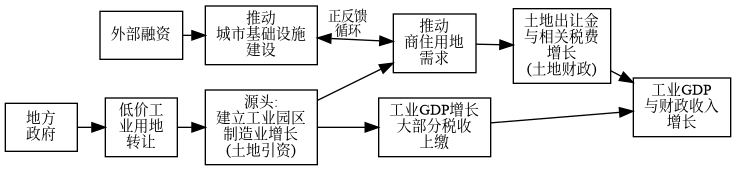
\includegraphics[width=0.9\textwidth]{figures/before08.png}
  \caption{\label{fig:bf08}2008年以前工业增长、土地财政与地区经济增长(可持
    续) }

  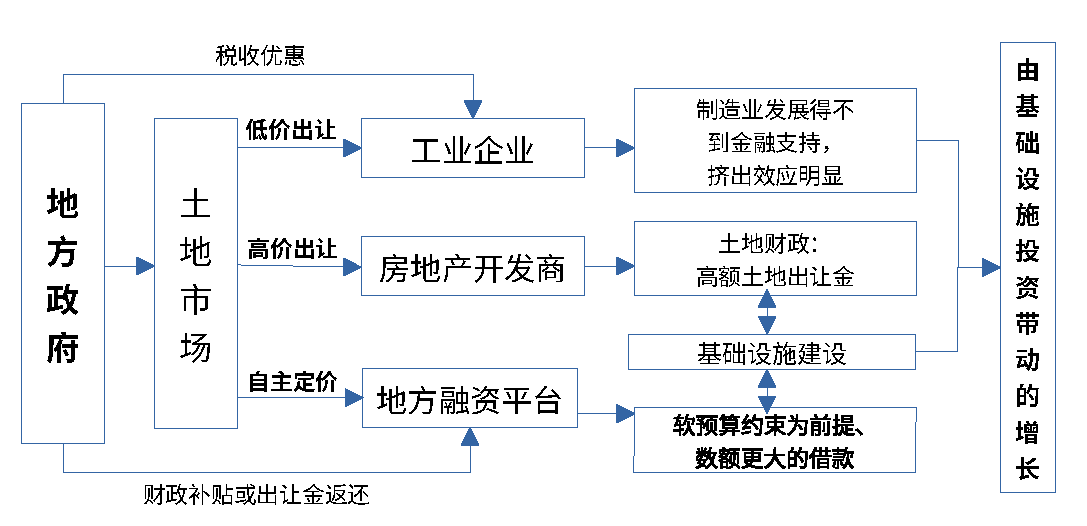
\includegraphics[width=0.9\textwidth]{figures/after08.pdf}
  \caption{\label{fig:af08}2008年后软预算约束与地区经济增长(不可持续) }
  \capsource{范剑勇\qquad《四万亿如何改变了中国经济增长动力》}
\end{figure}

据范剑勇\cite{fanjianyong}:
\begin{quotation}
  2008年之前,中国是硬预算约束条件的土地财政模式(见\cref{fig:bf08},而2008年
  之后,是软预算约束条件下的土地金融模式(见\cref{fig:af08}。2008年之前,经济
  增长的动力是“制造业+房地产”两个轮子一起转,2008年之后是偏向以基础设施为主
  的单轮驱动。
\end{quotation}

详细论述可见范原文,不再赘引。4万亿之后的土地金融历史,就本书所占角度来说,未发生
明显本质转变,也不再赘述。

\subsection{土地置换制度}

本小节几乎照摘周飞舟和谭飞智所著《当代中国的中央地方关系》。

自改革开放以来,我国工业化、城镇化推进速度越来越快,大量耕地农用地被占用是土
地财政\footnote{“土地财政”四字为笔者所加。}发展的必然要求。尤其是进入21世纪以来,
各地土地财政带来大拆大建,形成规模不小的失地农民群体,频发的群体性事件成为危
害社会稳定的重要因素。自中央层面来看,基于保障\textbf{国家粮食安全}以及维持改革以来
确立的家庭联产承包责任制的基本经营组织方式的要求,实行严格的耕地保护制度,以
占补平衡为代表的系列政策应运而生,\textbf{18亿亩耕地红线}作为一项政治任务贯穿而下,
实行一把手问责制。

\subsubsection{耕地占补平衡}

1997年4月,中共中央国务院发布11号文《关于进一步加强土地管理、切实保护耕地的通
知》,明确提出省(区市)必须保持耕地总量动态平衡的要求,同时确定了实行占用
耕地与开发复垦\footnote{土地复垦是指对生产建设活动和自然灾害损毁的土地,采取整治措施,
  使其达到可供利用状态的活动。}挂钩的政策,首次明确提出“耕地占补平衡”的概念。

随后在1998年8月,《中华人民共和国土地管理法》再次修订,明确提出“实行占用耕地
补偿制度”,要求占用耕地与开发复垦耕地相平衡。

1999年2月4日,《关于切实做好耕地占补平衡工作的通知》(国土资发〔1999〕39号)要
求确保建设占地“\textbf{占一补一}”,逐步实现耕地占用的\textbf{先补后占、占优补优、不补不
  占}。自此,耕地占补平衡政策开始在全国各地大规模实施。

2006年以前,占补平衡考核采取的是“\textbf{算大帐}”的方法——以区域为单位,考核区域内
的总占总补平衡。这种方法存在的漏洞是,很多建设用地项目并没有实现法律所规定的
占补平衡,建设用地占用耕地项目单位的补充耕地与土地开发整理脱钩。同时,由于区
域内的占补平衡考核仅仅关注于数量,一些建设项目\textbf{占优补劣}的现象比较突出。

2006年6月8日,国土资源部第3次部务会议通过了《耕地占补平衡考核办法》,于当
年8月1日起施行。“耕地占补平衡考核,\textbf{以建设用地项目为单位进行}”“耕地占补平
衡,实行占用耕地的\textbf{建设用地项目与补充耕地的土地开发整理项目挂钩}制度。”不再
采取大锅饭式的算大账。这一管理思路,为后来的增减挂钩所延续,即采用“\textbf{封闭运
  行}”的项目制运作模式,

随着工业化、城镇化的大势所趋,\textbf{“保耕地红线”成为地方政府沉重的政治负担和资金负
担。}耕地占补平衡政策自出台以来,在各地具体实施过程中主要存在:耕地的“\textbf{实占虚
补}”;补充耕地的“\textbf{实优虚劣}”以及\textbf{农地非农化和非粮化}的风险。耕地占补平衡制度实
行以来,各地实际工作中建设占用耕地长期以“先占后补”和“边占边补”方式为主,
加上对补充耕地的监督力度不够,导致建设占用耕地占而不补、占多补少的问题经常发
生。国土资源部因此颁布《关于进一步加强土地整理复垦开发工作的通知》,规定
从2009年开始,除国家重大工程可以暂缓外,非农占用耕地全面实行“\textbf{先补后占}”。

% 从地方政府角度出发,其更多的是从如何提高土地生产效益的角度出发的,因此如果单
% 纯地维持原有以粮食为主的种植结构难以达到提高效益的目的,转变生产结构成为必然
% 的选择,农地非农化、非粮化在所难免。所谓粮食安全的担忧也并非地方所考虑的问题。
% 在这一点上,中央与地方之间的矛盾凸显。

由于耕地的开垦整理需要一定的工程周期,因而由“先占后补”到“先补后占”的转变,
开启了\textbf{耕地占补平衡指标化}的进程,各地纷纷建立\textbf{占补平衡指标储备库}。提前储
备补充耕地,需新增建设用地时再从库中支取“指标”。

% 中国耕地红线粮食战略安全和土地金融的交织摩擦,使地区\textbf{狂热开发}建设用地的意
% 图受限\footnote{此句为笔者所加。以中国为一整体的角度来考虑,各地重复建设、大干快上,
% 工业用地扭曲的拿地或租赁价格、房地产的癫狂实属狂热无疑。},尤其是经济发达地
% 区与产粮大省更加受限于补充耕地资源较少。

% 从另一各方面来说,耕地红线也使可转化为新增建设用地的农地更加稀缺,加重了土地
% 金融的严重程度。\footnote{此句为笔者所加。}

\subsubsection{土地置换与指标折抵}

中央、省、市、县、乡五级政府的五级规划与年度建设占用耕地计划指标等限制了各级
地方政府对于新增建设用地、发展土地金融的强烈渴求,与中央严格土地制度框架出现
较尖锐矛盾,违法占地屡禁不止,中央政府为此开了以农用土地整理换取新增建设用地
的“口子”。

1999年10月,《国土资源部关于土地开发整理工作有关问题的通知》(国土资发
〔1999〕358号)提出土地置换和指标折抵。

\begin{description}
\item[土地置换] 促进农村居民点向中心村和集镇集中、乡镇企业向工业小区集中,选定新
  址\textbf{建设需要占用其他耕地}时,可以与腾出来的\textbf{旧址整理后增加的耕地}进行置换,实行
  这种方式置换的其建设用地\textbf{不占用年度建设占用耕地计划指标}。


\item[百分之六十指标折抵] 实现耕地占补平衡的地区,可以用通过土地整理\textbf{新增耕地面积
  的百分之六十指标},向上级土地行政主管部门申请一定数量的\textbf{预留建设占用耕地指标},
  用于本地区必需的非农建设。但必须按规划用地,并要严格检查,适当控制。
\end{description}

这两项政策“指标的使用并\textbf{不占用当年的年度建设用地指标},因而受到各地方政府的
欢迎……也是城乡建设用地增减挂钩政策出台的前奏”。

但地方政府仍感受到五级区域对于发展建设用地限制较大:发达地区可供补充耕地量匮
乏,不能满足新增建设用地需求;一般为10--15年的土地规划无法更好预见未来发展,
不可占用基本农田\footnote{基本农田:为了切实保护耕地,国家把按照一定时期人口和社会经
  济发展对农产品的需求,以及对建设用地的预测而确定的\textbf{长期或一定时期内不得占
    用的耕地}称为基本农田。}使大块建设用地项目难以落地。于是一些省开始省内跨
区域操作,实现了较为系统性变通的是浙江省,一些人称之为“\textbf{浙江模式}”。简而言
之就是浙江省将一些指标统筹在省或市以内,不下沉分解至各县各乡;并且各市之间可
以交易指标,落后地区大量土地整理用以补充耕地,发达地区向落后地区购买耕地指标
专心发展建设用地。详细了解可见汪晖、陶然《论土地发展权转移与交易的 “浙江模
式”——制度起源, 操作模式及其重要含义》。


\begin{quotation}
  对浙江在土地发展权转移和交易上的改革探索,不仅学界有论述质疑浙江的做法
  是\textbf{规避中央政府基本农田审批权和新增建设用地土地有偿使用费,导致基本农田质
    量下降和建设用地总量失控}(谭峻等,2004 年),中央政府也存在不少担心。

  欠发达地区为了折抵指标过度投资土地整理,甚至在新增耕地比例上弄虚作假,或发
  达地区通过购买折抵指标无限制扩张城市和工业园区用地。

  浙江省基本农田集中置换和易地代保政策\footnote{即基本农田易地代保:简而言之,发达市
    县有偿购买落后市县的基本农田,以便消除本市县相应面积、质量的基本农田保护,
    新增大块连续建设用地。}在国土资源部《关于进一步采取措施落实严格保护耕地制度的通
  知》(国土资发〔2003〕388 号和国务院办公厅《关于深入开展土地市场治理整顿严格
  土地管理的紧急通知》(国办发明电〔2004〕20 号)公布后停止执行;折抵指标政策也
  在《国务院办公厅关于严格执行有关农村集体建设用地法律和政策的通知》(国办发
  〔2007〕71 号)颁布后停止执行。\cite{wangzhejiang}
\end{quotation}


\todo[inline]{浙江模式其实就是市县级土地金融的扩大版,大国大城其实就是浙江模
  式的扩大版?参考LaTeX源文件中以下被注销部分。自由派认为行政主导要继续让位
  给市场自由流动。}

\subsubsection{城乡建设用地增减挂钩}

\begin{quotation}
  2004年10月21日国务院下发《关于深化改革严格土地管理的决定》,“实行最严格
  的土地管理制度……鼓励农村建设用地整理,\textbf{城镇建设用地}增加要与\textbf{农村建设用
    地}减少相挂钩”。

  (4年陆续增加试点后,)2008年6月27日,国土资源部印发《城乡建设用地增减挂钩
  试点管理办法》,明确提出了“城乡建设用地增减挂钩是指依据土地利用总体规
  划,\textbf{将若干拟整理复垦为耕地的农村建设用地地块(即拆旧地块)和拟用于城镇建
    设的地块(即建新地块)等面积共同组成建新拆旧项目区}(以下简称项目区),通
  过建新拆旧和土地整理复垦等措施,在保证项目区内各类土地面积平衡的基础上,最
  终实现\textbf{增加耕地有效面积,提高耕地质量,节约集约利用建设用地,城乡用地布局更
  合理}的目标。”其实仔细比较增减挂钩政策与之前我们所分析的建设用地指标置换政
  策其在表述上和本质上相类似,而这也反映了中国改革中政策制定的延续性和探索性。

  同时138号文批复下达了第二批试点项目(共10246公顷,合15.368万亩),项目区以
  项目区备选方式下达。2009年3月5日,《国土资源部关于2009年第一批城乡建设用地
  增减相挂钩周转指标的批复》(国土资函[2009]299号),对河北、内蒙古、辽宁、吉
  林、黑龙江、福建、江西、河南、湖南、广东、广西、云南、宁夏13省(区),批复
  下达周转指标15.275万亩(合10183.3公顷)。2013年10月23日下午,国土资源部部长、
  党组书记、国家土地总督察姜大明主持召开第15次部长办公会,审议并原则通
  过2013年城乡建设用地增减挂钩指标分解下达方案,共批准29个省份开展增减挂钩试
  点,全国共安排城乡建设用地增减挂钩指标90万亩。\cite{yangdi}
\end{quotation}

\begin{figure}[htbp!]
  \centering
  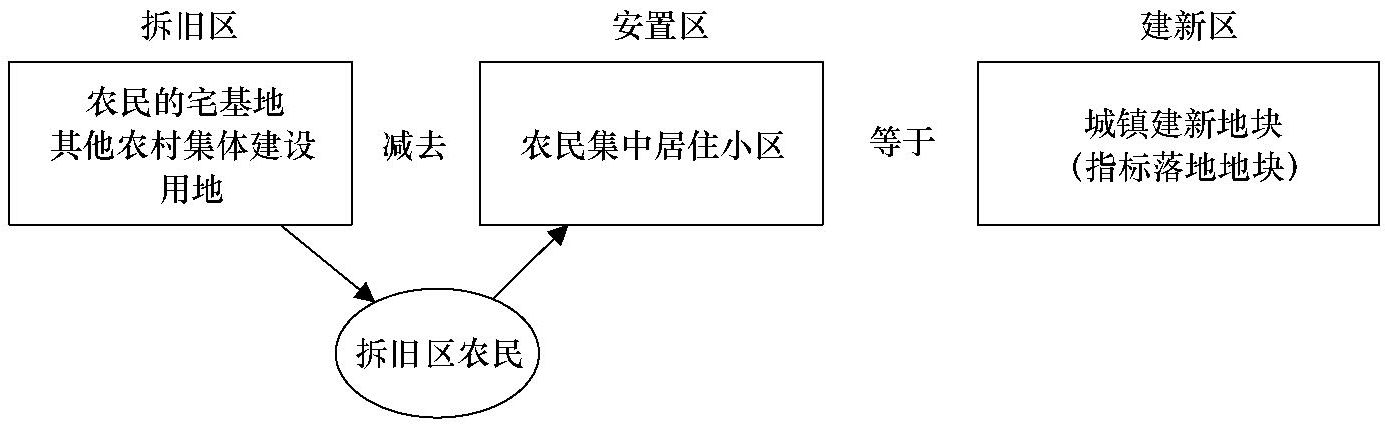
\includegraphics[width=0.9\linewidth]{figures/zengjianguagou.jpg}
  \caption{\label{fig:zengjianguagou}城乡建设用地增减挂钩政策示意图}
  \capsource{周飞舟、谭飞智\quad 《当代中国的中央地方关系》}
\end{figure}

\begin{quotation}
  指标计算公式:增减挂钩周转指标=拆旧区总面积-农民集中居住小区占地面积=项目区
  中建新地块可占地面积(见\cref{fig:zengjianguagou})。所谓“\textbf{周转指标}”其
  在实质上是一种指标“\textbf{预借}”或“\textbf{透支}”制度。拆旧复垦是一项非常庞大的工
  程,短期内难以完成,因此不需要拆旧区完成耕地复垦工作之后,建新区才能够进行
  城镇开发建设。也正是在这个意义上才有了指标“\textbf{周转}”的概念,一般要求,指标
  三年归还。

  增减挂钩的根本意义在于:开辟了一个独立于每年新增建设用地指标严控体系以外的
  指标来源,为城镇发展提供“不占指标”的“计划外”土地资源,且规模逐年增加。\cite{yangdi}


  截至2013年底,全国共有29个省(自治区、直辖市)被纳入了试点范围,共下达周转
  指标约90万亩。

  2017年4月,增减挂钩再出新政,在《关于进一步运用增减挂钩政策支持脱贫攻坚的通知》
  中,明确允许省级贫困县的增减挂钩节余指标在\textbf{省域范围内}流转使用,进一步释放了
  政策红利。为了落实国家乡村振兴战略,2018年3月,国务院办公厅印发了《城乡建设用
  地增减挂钩节余指标跨省域调剂管理办法》,规范了“三区三州”及其他深度贫困县增
  减挂钩节余指标\textbf{跨省域调剂},助力落实国家精准扶贫、绿色发展的战略。至此,增减
  挂钩先后两次完成政策升级,从省域内流转到跨省调剂,逐步拓展政策适用范围。这一
  阶段增减挂钩政策更加强调以人为本,致力于城乡区域协调发展和社会公
  平。\cite{zengjianzongshu}
\end{quotation}

据《央地关系》,不管是政策实质还是地方需求,对新增耕地并无多少刺激,只是满
足“占补平衡”即可。如\cref{fig:zengjianguagou},为获得更多新增建设用地,地方
倾向于减少农民集中居住小区占地面积,显而易见的方法是“农民上楼”——楼房可以
在单位占地面积提供更大容积率、容纳更多被增减挂钩析出的农民;并采用合村并居等
方法,以便进一步减少成本、扩大新增建设用地指标。

中央中央政府面临对地方监管失控的风险。一方面土地金融下,地方为GDP考核机制不满
足于中央给定的增减挂钩指标,为获得更多新增建设用地或直接将用地指标出售给其他地
方,对大量村庄违规改造;另一方面中央为维持地方发展的积极性及活力,又不得不逐
年扩大试点范围和规模。

增减挂钩以项目制方式向下推进,中央资金以项目形式向下转移,各级地方政府必须要
有相应的配套资金和政策支持,地方政府继续高额举债以及引入社会资本成为必然。债
务压力迫使地方忽视了反哺农业、农村、农民,仍倾向于以建设养建设;可同时进行的
拆旧和建新在极端情况下也会停滞或缓慢发展,造成各种不安定因素积累发酵;地方也
面临和社会资本的博弈;合村也带来更多政治管理矛盾。

起初农村拆迁矛盾多因行政强制指令下补偿不足,农地价征收城低价出售,城乡二元对
立有所加重,有损村民利益。随着政府日益重视农民权益问题,拆迁补偿已有较大实质
性改观。但随着市场经济边沁利己的日益深入人心,土地金融的日益发展,使土地成为
全民全社会共同参与的虚假繁荣市场,增减挂钩成本日益提高,越发加重了风险。


土地金融造成地方各自为政,产业结构相同且全副该,重复建设,狂热追求新增建设用地,农民上楼,大额投资等等


% 韩长赋: 中国农村土地制度改革

% 耕地退化、污染严重,一些地方占好地、补坏地,占水地、补旱地,2016 年全国优高
% 等耕地面积仅占 29. 5%。




% 反面论述
% https://www.aisixiang.com/data/115819.html
% 赵燕菁:从土地金融到土地财政:资本的胜利、有为的政府与城市的转型

% ※※※※※※※※※※※※※※※※※※※※※※※※※※
% https://bfi.uchicago.edu/wp-content/uploads/2022/02/BFI_WP_2022-24.pdf

% 文献中的典型观点是,住宅用地出让主要是地方政府增加收入的一种方式,而工业用地
% 出卖主要是为了补贴产业、刺激经济增长、支持劳动力需求。

% 中国的土地市场具有相当大的工业折扣:工业区用地比住宅用地便宜一个数量级。与以
% 产业补贴或促进产业增长为中心的解释相反,我们强调了未来土地税收的重要性,并发
% 现地方公共财政激励措施可以在很大程度上合理化这种价格差距。在“土地融资”制度
% 下,土地出让是中国地方政府的重要收入来源。研究表明,在中国,地方政府作为垄断
% 性土地销售者,面临着住宅用地或工业用地供应之间的权衡,这取决于工业和住宅用地
% 销售收入的不同时间分布、地方政府的财政约束以及地方政府与其他各级政府分享税收
% 的程度。

% 公司税收收入和土地出让收入;2019年,这两个数字分别约为8.7万亿元人民币和7.3万
% 亿元人民币.2工业用地产生持续的未来税收流动,因为工业企业缴纳增值税和所得税,
% 以及各种费用。由于中国没有住宅物业税,住宅用地销售只会暂时增加房屋开发商缴纳
% 的税款.3这意味着地方政府面临着一个选择,即出售前期收入较大的住宅用地和出售工
% 业用地,因为工业用地支付的税收现金流比实际收入更持久。

% 这种动态的观点意味着,大量的前期工业用地折扣并不一定意味着政府正在通过廉价土
% 地系统地补贴工业。事实上,我们表明,在调整住宅开发商缴纳的税款后,来自工业用
% 地的税收流动可以定量补偿前期工业用地折扣。我们还提供了地方政府的融资需求影响
% 土地分区的因果证据,表明地方公共财政在通过土地分配渠道塑造中国经济增长路径方
% 面发挥着被低估的作用

% 我们从一个概念框架开始,分析推动工业用地而不是住宅用地供应均衡回报的力量。我
% 们考虑的是地方政府,其目标是最大化其财政收入的现值。除了全部属于地方政府的前
% 期土地销售收入外,住宅用地还产生了由房屋开发商支付的一次性税款,而工业用地则
% 产生了工业税的持续现金流,并与中央政府共享。在均衡状态下,由于未来的税收优惠,
% 当地政府愿意以较低的价格出售工业用地。该框架指出了两个简单且可衡量的汇总统计
% 数据。首先是工业折扣,即工业用地和住宅用地之间的价格差异。第二种是工业用地销
% 售的内部收益率(IRR),计算为贴现率,折现率等于工业和住宅用地销售的所有现金
% 流的现值

% ※※※※※※※※※※※※※※※※※※※※※※※※※※

% 就像许多其他国家一样,中国也有严格的分区限制。正如Chen等人(2018)所强调的那
% 样,划为住宅用途的土地的售价大约比划为工业用途的土地高出十倍。2019年,中国住
% 宅用地平均价格为3,619元/平方米,工业用地平均价格为304元/平方米。我们将住宅用
% 地和工业用地之间的这种价格差异称为工业用地折扣(或工业用地互换)。

% ※※※※※※※※※※※※※※※※※※※※※※※※※※

% 地方政府从土地中获取融资有两条直接渠道:一是土地财政,即通过出让国有土地(主
% 要是商服用地和住宅用地)50至70年的使用权来获取级差地租;二是土地金融,即将土
% 地注入地方融资平台来撬动资金为城市建设融资。

% 已有研究表明,土地财政和土地金融相结合的以地融资模式催生出一个高效的融资体系,
% 极大推动了近二十年来的中国经济增长,特别是与房地产和基建相关(包括钢铁、水泥)
% 的重工业部门得到了飞速发展,居住环境和基础设施的改善又进一步促进了地价和房价
% 的升值,为下一轮以地融资创造了有利条件。这样的正向反馈机制使得中国自1998年以
% 来一直处于投资驱动型的增长阶段。

% 如果说曾经的以地融资模式主要依赖土地财政,那么如今,随着部分地区土地资源的告
% 罄和征地补偿标准的提升,一些地方政府对土地财政的依赖开始减退,而对土地金融却
% 愈加青睐。由表1可知,越是土地资源稀缺的地区(东部地区),土地抵押贷款规模越
% 是高于土地出让规模,而对北上广这样的一线城市而言,土地抵押与土地出让的比值更
% 是高于东部地区的平均水平。

% 图1显示,2003至2010年间,出让成本占比基本维持在六成左右,但在2011至2018年间,无论是土地出让成本的规模还是其占土地出让毛收入的比重都呈加速上升趋势,甚至到了2018年,土地出让成本占土地出让毛收入比重已接近九成。

% 从征地规模的角度亦可佐证土地出让成本在2010年前后出现了飘升的现象。图2显示,农用地和总的土地征收规模在2011年之前处于上升区间,但在2011年后呈逐年加速下滑的态势,这恰好是土地出让成本开始飘升的年份(参见图1)。迅速缩小的征地规模表明,未来国有土地的出让规模将大幅缩减,利用土地财政进行创收的空间将被进一步压缩。

% 1994年的税收分享改革,该改革减少了地方政府在许多税收收入来源中的份额,同时并没有减少他们的支出需求。要回答“为什么土地金融在中国(到目前为止)有效运作”要复杂得多。在这方面,了解其促进土地金融体系盈利能力的制度基础是很重要的。首先,地方政府被指定为地方城市LUR的垄断提供者。因此,当一个城市提出购买农村土地并将其转换为城市土地时,它不会面临来自其他实体的竞争。此外,支付的补偿是基于当前(农业)用途的土地价值,而不是未来城市用途。地方政府回购、分配或出售的城市土地利用率并将其转换为新的土地利用率时,也适用类似的规定。这种安排使城市政府能够获利,直到最近,土地价格的暂时上升趋势加剧了这一点。值得注意的是,支撑土地金融体系的丰富制度框架既有法律、官方文件等显性规则,也有在实践中具有影响力的隐性规范。其中一些细节在现有文献中似乎没有得到适当的承认,并可能导致对该系统的误解。希望我们的分析能够更清楚地说明该系统在中国联邦体系中的运作方式

% 自1980年代以来,中央和地方政府在中国经济中扮演的角色已经很明确——中央政府负责规划和监管,而地方政府则负责在地方层面实施这些法规。

% 从1980年到2020年,地方政府在国家一般公共预算中的份额从45.7\%增加到85.7\%,而同期收入在一般公共预算中的份额从75.5\%下降到55.5\%。为了弥补收支缺口,地方政府依靠中央政府补贴、债务融资和土地融资。

% 1994年实行的税制改革在随后的几年中对土地融资产生了巨大的溢出效应。改革规定,中央政府将把所有与土地有关的税收分配给地方政府。这包括土地价值税、城市土地使用税、耕地占用税、土地增值税、契税(财产转让税)和一般财产税。更重要的是,土地出让的所有利润都转移到了地方政府。

% 这一新制度为地方政府增加了土地出让收入提供了强大的动力。从2000年到2020年,地方政府土地出让收入占总收入的比重从5.9\%提高到42\%。如果将其他相关的土地税也考虑在内,土地收入占地方政府总收入的一半以上(52\%)。

% o“通过信用制度,未来的收益可以贴现到今天,使得资本的形成方式得以摆脱对过去积累依赖,转向预期收益。”“中国城市伟大成就背后的真正秘密,就是创造性地发展出一套将土地作为信用基础的制度——‘土地财政’。”


% 土地财政是指政府出让国有土地使用权收入,及与土地有关的税收如耕地占用税、土地增值税等,这都是有法律、制度依据的。土地金融是指政府拿土地做抵押,向银行贷款,属于政府负债。这样做,没有法律依据,是打了制度的“擦边球”,因为制度允许政府作为国有土地所有权的代表经营土地。


% 但是当市场经济更多要求个人为个人负责,并将此观念植入人心时,一些原住民的死缠
% 烂打、坐地起价也就避无可避,因此拆迁往往要大费周章。突破口似乎只有合法或非法
% 的“暴力”。

% 合法暴力,可以宣称土地权利不归属于抗拒拆迁的人员,如印度最高法院声称孟买等地
% 贫民窟的长期居民是土地的非法占有者,没有权利要求拆迁赔偿,\textbf{承认获赔权等于奖
% 励盗窃行为};美国滥用征地权,把合理建筑中的长期居民赶走,鼓励高层建筑;声称
% 土地为集体所有,集体才是土地权利所有者,而非小部分人。

% 非法暴力,如20世纪90年代韩国首尔开发商雇佣黑帮“相扑似的打手”暴力拆迁;印度
% 西孟加拉邦南迪格莱姆地区的冲突惨案等。


% 《从沸腾到癫狂》

% 北京2005~2009年政府公布的商品房住宅建设用地计划供给指标为7130公顷,非商品住
% 房建设用地指标为1320公顷,两者的比重为5.4∶1。而实际供给的情况则是,商品房住
% 宅用地(招拍挂)2394公顷,完成计划数的33.6%,供地差额为4736公顷;非商品住宅
% 供地1283公顷,完成97.20%,扣除商品房中的配建,非商品房完成率为103%。这些土
% 地为享受经济适用住房政策的用地,约为商品房用地的2倍,由特定单位使用了。商品住
% 宅用地与非商品住宅用地的面积相加,可以计算出商品住宅用地在全部住宅建设用地中
% 的比重仅为28.3%。



% 任志强认为,市场中计算出的商品住宅平均销售价格仅为这28.3%的住宅销售价格,而并非北京市的住宅实际价格。如果用地中的平均容积率相等,且大部分经济适用住房和享受经济适用住房政策的住房价格为4500元/平方米,则北京市的一手房销售价格约仅为6200元/平方米。

% 任志强说,虽然那些低价的定向住房没有向社会公开销售,比如分给了国务院事务管理局,再分配给中央或国务院的各机关、管理机构以解决公务员的住房、进京干部的住房、老干部的住房等,但这些住房也是解决北京的住房问题,所以,应该在统计时计算进来进行平均。

% 房真实房价平均仅为6200元/平方米。而根据北京市统计局、国家统计局北京调查总队公布的《2009年北京市房地产市场运行情况》,2009年第四季度,四环路以内商品住宅期房销售均价为25907元/平方米。

% 6200元/平方米与25907元/平方米,为什么两者的差距如此之大?



% 任志强如是写道:



% 北京2005~2009年政府公布的商品房住宅建设用地计划供给指标为7130公顷,非商品住房建设用地指标为1320公顷,两者的比重为5.4∶1。而实际供给的情况则是,商品房住宅用地(招拍挂)2394公顷,完成计划数的33.6%,供地差额为4736公顷;非商品住宅供地1283公顷,完成97.20%,扣除商品房中的配建,非商品房完成率为103%。这些土地为享受经济适用住房政策的用地,约为商品房用地的2倍,由特定单位使用了。商品住宅用地与非商品住宅用地的面积相加,可以计算出商品住宅用地在全部住宅建设用地中的比重仅为28.3%。



% 任志强认为,市场中计算出的商品住宅平均销售价格仅为这28.3%的住宅销售价格,而并非北京市的住宅实际价格。如果用地中的平均容积率相等,且大部分经济适用住房和享受经济适用住房政策的住房价格为4500元/平方米,则北京市的一手房销售价格约仅为6200元/平方米。

% 任志强说,虽然那些低价的定向住房没有向社会公开销售,比如分给了国务院事务管理局,再分配给中央或国务院的各机关、管理机构以解决公务员的住房、进京干部的住房、老干部的住房等,但这些住房也是解决北京的住房问题,所以,应该在统计时计算进来进行平均。

% 按照任志强的说法,商品住宅用地28.3%之外的用地,一部分被用于建设北京市和在京中央和国家机关的公务员住房,他们的名称可以是两限房、经济适用住房、享受经济适用住房政策的住房、合建房、自建房中的任何一个。当然,也不排除这些公务员在享受了经济适用房等保障房以后,仍然自掏腰包去购买商品房。



% 地产商什么时候成为一个阶层了?正统的社会学者肯定要嘲笑我的无知。他们会教育我:你可以称他们为一个群体,一个集团,就是不能称其为一个阶层。是啊,连天天挂在老百姓嘴边的“中产阶层”都未获正式承认,哪里来的地产商阶层?

% 为什么地方政府会产生对土地财政像网瘾一样的依赖?根子在于土地招拍挂制度。这是一个影响力仅次于1998年房改的制度,并将继续对房地产市场和地方财政产生决定性的导向作用。

% 招拍挂制度必然导致地价上涨,而地价上涨则必然推动房价上涨。只要招拍挂制度存在,地王的产生就不可避免。地产GDP主义是被一种强力制度牢牢地固定住的地方政府价值取向。

% 并于2010年6月后成功超过日本成为全球第二大经济体,其中房地产贡献良多。据国家统计局数据,2010年,全国房地产开发投资完成48267亿元,同比增长33.2%;全国商品房销售面积10.43亿平方米,同比增长10.1%;商品房销售额约为5.25万亿元,同比增长18.3%。

% 因此,即使是全面调控的2010年,房地产的地位也丝毫没有下降。自从1998年实行住房商品化以后,GDP对房地产业的依赖就逐步形成,以至于到了离不开的地步,关键时刻总是要靠房地产“挺身救主”。实事求是地说,这方面没有一个产业能比得上房地产。

% 以上是从全局,从中央政府层面来说。对地方政府来说,房地产就更重要了。土地财政,这已成为大多数地方政府最重要的财政收入来源。城市形象、政绩工程也离不开地产商和房地产业,许多地方的道路等基础设施都是由地产商修建的。

% 2004年以来,地方政府体会到土地公开出让的无可替代的好处,招拍挂出让普遍推行。而招拍挂一般是净地出让,拆迁是政府的事。而土地收益当然要远大于拆迁补偿款,否则他们是没动力拆的。地方政府为了尽快把土地卖出去,就会做出强制拆迁、暴力拆迁的事情来。


% 1991年实施和2001年修改的《城市房屋拆迁管理条例》。依此条例,地方政府贴一纸拆迁通知,在被拆迁的房屋上圈画一个大大的“拆”字就够了。居民不肯搬迁?先有房管部门行政裁决强制拆迁;还不服?接着可能就是法院裁决直接带着铲车来。许多地方连行政和法院裁决都懒得走,直接派消防队和铲车来。这才叫雷厉风行,超级效率。中国城市面貌的日新月异,城市建设的突飞猛进,该《条例》立了大功。

% 不少专家称这部条例是一部恶法,出台伊始就呼吁修改之。修改后的条例草案数易其稿,并分别于2010年1月29日和12月15日分两次向全社会公开征求意见,这在我国立法史上前所未有,也从一个侧面证明了拆迁所涉及的利益极为纷繁复杂。北大法学教授说,新的条例难以正式出台,主要就是遭遇到地方政府的强烈阻挠。千呼万唤之后,2011年1月21日,国务院正式出台《国有土地上房屋征收与补偿条例》。



% 2007年1月,国家税务总局曾要求各地税务机关严格土地增值税清算,此举曾令开发商大
% 为紧张。然而,金融危机呼啸而来,经济形势急转直下,这一号称“革房地产商命”的
% 税收政策再一次不了了之。赵晓等吁请严征土地增值税,以“100%预征、100%清
% 算”来遏制新一轮楼市疯狂。

% 到遏制投机的作用一样,对地产商和投资者个人尤其是地产商征收土地增值税,亦未能成为阻止涨价的动力。

% 事实上,土地增值税更像是为地方政府找到了一个新的税收来源,虽然这可能并非该税种设立的初衷。

% 严格征收土地增值税,能够为地方政府带来多大的税收?实事求是地说,2010年以来的保障房建设规模,令人惊讶。

% 很难想象,如果没有2008年10月推出的4万亿政府投资计划,保障房建设会有今天如此庞大的规模。我并不是说加快保障房建设是为了应对国际金融危机而采取的措施,而是说,保障房建设规模如此庞大,沾了4万亿“救市”资金的光。

% 2008年11月5日召开的国务院常务会议,确定了进一步扩大内需、促进经济增长的十项措施(“出手要快,出拳要重”的说法由此而来),第一条就是加快建设保障性安居工程。在4万亿投资里,坊间曾有保障房占8000亿元、9000亿元的说法,但并不准确。

% 根据国家发改委主任张平2009年3月8日在十一届全国人大二次会议新闻发布会的介绍,在4万亿政府投资计划中,保障性住房投资总规模为4000亿元左右。从张平的介绍来看,保障房包括廉租房、林区、垦区、煤矿棚户区改造,但没有提到限价房、经济适用房、公共租赁房等的投资,所以实际投资规模要远远大于4000亿元。

% 2008年受国际金融危机影响,除北京等极个别城市外,各地对保障房投入仍然不足。真正较大规模的保障房建设是从2009年开始的。

% 根据2010年3月5日全国“两会”上的《政府工作报告》,2009年中央财政安排保障性安居工程补助资金551亿元,比上年增长2倍。新建、改扩建各类保障性住房200万套,棚户区改造解决住房130万套。从中央财政投入看,增幅甚大。那么,2009年地方对保障房的投入有多少呢?

% 全国人大常委会专题调研组2009年10月月底披露的一份调查报告显示,截至当年8月月底,全国保障性住房建设完成投资394.9亿元,完成率仅为23.6%。以此推算,当年全国保障房投资计划大约为1600亿元。减去中央财政投入的551亿元,地方即使足额完成投入计划,亦不过1050亿元。

% 财政部2007年11月颁布的《廉租住房保障资金管理办法》规定,应从土地出让净收益中按照不低于10%的比例安排用于廉租住房保障资金。2009年全国土地收益实际到账14239亿元。也就是说,2009年各地仅廉租房就应投入1424亿元。加上公共租赁房、经济适用房和限价房,总投入至少应该倍增。而事实上,2009年各地保障房实际投入额尚不足财政部规定的廉租房投入额,遑论加上公共租赁房、经济适用房和限价房。

% 当然,从全国“两会”《政府工作报告》公布的数据看,2009年全国保障房建设任务是完成了的。330万套保障房的投资,应远远超过1600亿元。

% 2010年的保障房建设规模更加惊人。根据住房和城乡建设部的安排,2010年全国计划建设廉租住房、公共租赁住房等300万套,改造各类棚户区住房280万套,农村危房改造试点120万户。农村危房改造不计,人们将2010年的保障房任务简称为580万套。从330万套,到580万套,增长超过70%。

% https://www.mof.gov.cn/zhuantihuigu/czjbqk2011/czsr2011/201208/t20120831_679821.html
% 全国土地出让收入管理及使用情况

% 2007年之前,土地出让收入先纳入预算外专户管理,再将扣除征地补偿和拆迁费用以及
% 土地开发支出等成本性支出后的余额缴入地方国库,纳入地方政府性基金预算管理。
% 从2007年开始,国家对土地出让收入管理制度进行了改革,将全部土地出让收入缴入地
% 方国库,纳入地方政府性基金预算管理,与公共财政预算分开核算,专款专用。土地出
% 让收支纳入政府性基金预决算编制范围,实行预决算管理制度。每年第三季度,国土资
% 源管理等有关部门按照相关规定编制下一年度土地出让收支预算。每年年度终了,国土
% 资源管理等有关部门按照规定编制上年土地出让收支决算。同时,按照规定程序向同级
% 人民政府报告,政府依法向同级人大报告。

% 新自由主义,彻底的附庸
% 杨继绳《中国改革时代的政治斗争》
% \begin{quotation}

% 新左派认为,目前中国的改革越来越走向自由主义所倡导的模式,中国正在进入资本主义全球体系。当前“中国社会的各种行为,包括经济、政治和文化行为甚至政府行为,都深刻地受制于资本和市场活动。”“80年代中国的启蒙思想所许诺的‘好社会’不仅没有伴随经济市场化而到来,市场社会本身呈现了新的、在某种意义上来说是更加难以克服的矛盾。”(汪晖:《当代中国思想状况和现代性问题》)新左派满怀忧虑地问道:“我们今天这个世界究竟是谁在统治,是人民呢还是寡头?是权力呢还是资本?这是需要深思的。在全球化潮流下,跨国公司正在系统地、有步骤地剥夺世界各国人民的民主权利,正在把我们这个世界带向奴役之路。如果看不到这一现实的威胁,恐怕就谈不上懂得民主。“(韩德强,2000)

% 自由派认为,目前中国虽然存在种种问题,但正在从不合理的体制走向合理的体制,走向人类文明的主流。他们所说的人类文明的主流就是以英美为标志的价值体系和社会制度。“对于自由主义立场而言,中国向市场经济转型问题再多再严重,也只能硬着头皮向前走,决不能走回头路,决不能返回衣、食、往、行都被人包办,种什么,造什么,卖什么都得等上级指示的那种日子。”(徐友渔:《自由主义与当代中国》)

% 对当前的社会结构的变化,自由主义者持乐观的态度。他们认为,20年的改革,已经在政府之外开始出现了新的社会结构,这种新的社会结构可能是将来中国的市民社会和公共领域的雏形,在中国的社会发展中是将成为一支重要力量。因此,让这种新的社会结构进一步发展是一条必由之路。新左派认为上述看法是当今既得利益集团虚构的神话,他们认为,这20年所形成的不是中间阶层,而是新生的资产阶,是垄断精英,垄断精英是改革中社会不公正的既得利益者,是需要限制的、而不是应当鼓励发展的阶层。

% 中国正处在十字路口,搞得好,就可能建成一个民主、法治的社会,搞不好,就可能形成一个金权、家庭统治的新型专制制度。就像某些南亚和拉美国家一样。这是两派一致的看法。但是,新左派认为这种危险在于市场霸权和垄断精英,自由主义者认为这种危险在于没有得到改革的原有的权力结构,在于中国两千多年相沿成习的专制主义。

% 自由主义者把政治权力的无限膨胀看成是奴役民众的力量,新左派把市场力量的无限膨胀看成是奴役民众的力量。
% \end{quotation}


% #+BEGIN_SRC dot :file before08.png :cmdline -Kdot -Tpng :exports results
%   digraph G {
%     rankdir="LR"
%     rank=min
%     ranksep=0
%     node[shape=record fontsize=11]
%     yuan[label="源头:\n建立工业园区\n制造业增长\n(土地引资)"]
%     shangzhu[label="推动\n商住用地\n需求"]
%     jishe[label="推动\n城市基础设施\n建设"]
%     end[label="工业GDP\n与财政收入\n增长"]
%     gongshui[label="工业GDP增长\n大部分税收\n上缴"]

%    外部融资 ->  jishe
%    jishe -> shangzhu[dir=both, label="正反馈\n循环", fontsize=10]
%    shangzhu -> "土地出让金\n与相关税费\n增长\n(土地财政)" -> end

%     "地方\n政府" -> "低价工\n业用地\n转让" -> yuan -> gongshui ->end

%     yuan -> shangzhu
%     {rank=same gongshui  shangzhu}
%   }
% #+END_SRC

%%% Local Variables:
%%% mode: latex
%%% TeX-master: "../main"
%%% End:
